% mainfile: ../../main.tex
\chapter{Photoluminescence and excitons in semiconductors}\label{ch:exp:theory}
% TODO: wider introduction of PL in semiconductors before going towards doping
\AutoLettrine{The} development of remote-doping techniques enabled the growth of extremely high-mobility \glspl{2deg} in \GaAsAlGaAs heterostructures~\cite{Ihn2009}.
In these structures, dopants are introduced into the \ch{AlGaAs} barrier layer some \qty{50}{\nano\meter} away from the \ch{GaAs} layer and thus spatially separated by a \ch{AlGaAs} spacer layer.
This reduces Coulomb scattering in the \gls{2deg} induced by the doping and produces very high-quality samples as evidenced for example by the observation of the fractional quantum Hall effect~\cite{Stormer1999a}.
It is hence not at all surprising that early quantum dot experiments also took place in this well-understood material system.
While undoped approaches to electron and hole spin qubits in \ch{GaAs} exist~\cite{Harrell1999,Chen2012,Li2014,Tracy2014}, they introduce added complications because of the need to electrostatically induce a \gls{2deg} and reliably contacting it~\cite{Rossler2016}.
What is more, these issues are exacerbated when the structures need to be thinned down to a membrane~\cite{Descamps2021,Kindel2025}.
Therefore, to accommodate \glspl{gdqd} next to the \gls{oaqd} in the membrane, the devices measured in \thispart are fabricated on doped heterostructures hosting a \gls{2deg}.
In the following, I discuss the optical behavior of these structures under illumination.\sidenote{
    The \emph{electrical} behavior is another matter; there, illumination can lead to the creation, trapping, and de-trapping of free charge carriers that alter the transport properties of the device, leading to electrical hysteresis and instability~\cite{Fujita2021,Shetty2022,Wang2023,Reznikov2024,Kindel2025}.
}

\section{Photoluminescence in doped \GaAsAlGaAs heterostructures}\label{sec:exp:theory:pl}
\begin{marginfigure}
    \centering
    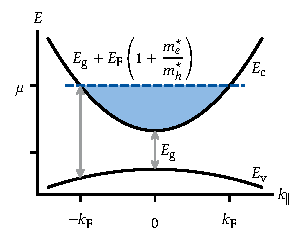
\includegraphics{img/pdf/experiment/2deg_sketch}
    \caption[\imgsource{img/py/experiment/pl.py}]{
        Band structure diagram of a doped heterostructure (after \citer{Kamburov2017}).
        Due to the $n$-type doping, the conduction band is filled up to the Fermi level $\mu$.
        Photonic excitation of an electron-hole pair can only occur at $\abs{k} > k_\mr{F}$ into the free states above $\mu$ due to the small photon momentum.
        Recombination can occur within a bandwidth of $E_\mr{F}(1 + m^\ast_{\mr{c}}/m^\ast_{\mr{hh}})$.
    }
    \label{fig:exp:theory:bandstructure:doped}
\end{marginfigure}
Consider an intrinsic, direct-gap, Zincblende semiconductor such as \ch{GaAs} with a band gap of $E_{\mr{g}} = \qty{1.519}{\electronvolt}$ at zero temperature~\cite{Vurgaftman2001}.
At the $\Gamma$-point, the conduction band is well approximated by a parabolic band with effective mass $m^\ast_{\mr{c}}/m_{\mr{e}} = 0.067$ and is offset by $E_{\mr{g}}/2$ above the Fermi level $\mu$.
Offset by the same absolute amount in the opposite direction is the valence band, which close to $\Gamma$ is fourfold degenerate with heavy and light holes with effective masses $m^{\ast}_{\mr{hh}}/m_{\mr{e}} = 0.34$ and $m^{\ast}_{\mr{lh}}/m_{\mr{e}} = 0.09$, respectively~\cite{Miller1984a}.
The third valence band\sidenote{
    The valence bands are $p$-like and hence contain contributions from three twofold degenerate atomic orbitals.
}
is split off by the spin-orbit interaction and lies \qty{0.34}{\electronvolt} below the other valence bands~\cite{Davies2009}.
Introducing confinement in one direction, for example by doping a \GaAsAlGaAs heterojunction or growing a \ch{GaAs} \gls{qw} sandwiched between two layers of \ch{AlGaAs}, lifts the fourfold degeneracy of light and heavy holes and leaves -- under usual conditions -- the latter as the valence band ground state.

Doping in sufficiently high concentration then raises the Fermi level from mid-gap to inside the conduction band in the plane of confinement, resulting in a band structure as sketched in \cref{fig:exp:theory:bandstructure:doped}.
The bands remain parabolic as function of the in-plane wave vector $k_{\parallel}$ close to $\Gamma$.
The conduction band is filled up to $\mu$ where, measured from the conduction band edge, $E_{\mr{c}}(k_{\parallel} = k_{\mr{F}}) = E_{\mr{F}} = \hbar^2 k_{\mr{F}}^2/2m^\ast_{\mr{c}}$ with the Fermi wave vector $k_{\mr{F}}\sim\qty{1e8}{\per\meter}$.
Now, absorption of a photon incident on the semiconductor demands conservation of energy and momentum.
The latter condition implies that hole and electron have close to equal momentum because $k_{\gamma} = 2\pi/\lambda\approx\qty{8e6}{\per\meter}$ is much smaller than $k_{\mr{F}}$.
Thus, excitation of an electron-hole pair from the valence into the conduction band occurs only for $k\geq k_{\mr{F}}$.
By contrast, recombination can take place for any $k$ in principle.
In practice, however, photo-electrons quickly relax down to the Fermi level, and recombination takes place between electrons inside the Fermi sea and photo-holes somewhere in the valence band at $k\leq k_{\mr{F}}$.\sidenote{
    For sufficiently localized states in real space, a wide range of $k$ states in the valence band is available for recombination as states are extended in $k$-space.
    We can estimate the localization length required for states up to $k_{\mr{F}}$ to participate by $\Delta x \geq\flatfrac{1}{2\Delta k} = 1/2k_{\mr{F}}\sim\qty{5}{\nano\meter}$ for a typical \gls{2deg}.
}
The former condition then implies $E_{\gamma} \geq E_{\mr{g}} + E_{\mr{F}}\left(1 + m^{\ast}_{\mr{c}}/m^{\ast}_{\mr{hh}}\right)$ because no free electron states are available in the conduction band below $\mu$ due to the Pauli exclusion principle and where the term in parentheses is due to the valence band dispersion.
Many-body effects due to localized photo-holes scattering with electrons of the Fermi sea can lead to a strong enhancement of luminescence intensity at the Fermi edge, the so-called \gls{fes}~\cite{Mahan1967,Mahan1967a,Skolnick1987}.
The intensity of the \gls{pl} at the Fermi edge relative to recombination at the band edge ($k_{\parallel} = 0$) is thus an indicator of the \gls{qw} interface quality and degree of alloy fluctuations, both of which lead to hole localization~\cite{Melin2000,Gabbay2008}.

Free electron-hole pairs created by photo-excitation can form hydrogenic bound states due to the Coulomb attraction of their opposite electric charges, \emph{excitons}.
In two dimensions, this effect is strongly enhanced due to the increased overlap of electron and hole wave functions.
Furthermore, the reduced dimensionality also enhances the binding energy from $\sim\qty{4}{\milli\electronvolt}$ in bulk \ch{GaAs} to up to four times that in \ch{GaAs} \glspl{qw}~\cite{Andreani1990,Gilliland1997}.
Rather than the continuum of the joint density of states of valence and conduction band discussed previously, excitons are discrete states whose energy is lower than the band gap energy by the binding energy, $E_X = E_{\mr{g}} - E_{\mr{b}}$.
In doped \glspl{qw} hosting a \gls{2deg}, the free carriers can screen the exciton binding energy and lead to an ionized electron-hole plasma~\cite{Palmieri2020}.
This is known as the insulator-to-metal (Mott) transition in semiconductors~\cite{Mott1968}.
Competing with this are so-called Mahan excitons~\cite{Mahan1967,Mahan1967a} that give rise to the \gls{fes}~\cite{Schleife2011}.

Next, I discuss the influence of an electric field on excitons.
For this, we return to undoped structures for simplicity.

\section{The quantum-confined Stark effect}\label{sec:exp:theory:qcse}
\begin{marginfigure}
    \centering
    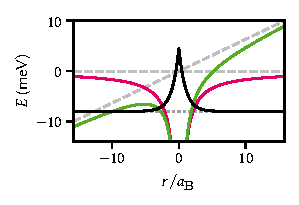
\includegraphics{img/pdf/experiment/in_plane_field}
    \caption[\imgsource{img/py/experiment/qcse.py}]{
        Effect of an in-plane electric field on an exciton wave function.
        In the hole's reference frame, the electron sees a static attractive Coulomb potential (magenta), resulting in a bound state (dotted gray line, wave function sketched in black).
        Applying an electric field ($F=\qty{100}{\milli\volt\per\micro\meter}$, dashed gray lines) tilts the Coulomb potential (green) and leads to a transparent barrier through which the electron can tunnel out.
    % In-plane fields -> field ionization -> line broadening \cite{Miller1985}
    }
    \label{fig:exp:theory:in_plane_field}
\end{marginfigure}

Consider the electron-hole pair in bulk \ch{GaAs} in the co-moving frame of the hole.
The hole generates the Coulomb potential
\begin{equation}
    V(r) = \frac{e}{4\pi\eps_0\eps_{\mr{r}}\abs{r}},
\end{equation}
where $\eps_{\mr{r}} = \num{13.3}$ is the relative permittivity of \ch{GaAs} at low temperatures, which attracts the electron by the Coulomb energy $E(r) = qV(r) = -eV(r)$.
\Cref{fig:exp:theory:in_plane_field} depicts the Coulomb potential in magenta and the bound electron's wave function sketched in black.
The electron-hole separation $r$ is shown in units of the exciton Bohr radius in two dimensions~\cite{Olsen2016}
\begin{equation}
    a_{\mr{B}} = \frac{2\pi\eps_0\eps_{\mr{r}}\hbar^2}{\mu e^2} = \qty{6}{\nano\meter}
\end{equation}
with $\mu$ the reduced effective mass of conduction and heavy-hole valence bands.

We now apply an electric field $F$.
This modifies the potential seen by the electron by $erF$ as sketched in green \cref{fig:exp:theory:in_plane_field}.
Ignoring changes to the electron wave function, we can see that the electron can tunnel out of the Coulomb potential, leading to \emph{field-induced ionization} of the exciton.
Now place the exciton in a \gls{qw} instead of in bulk with the electric field pointed such that it is out-of-plane of the \gls{qw}.
The field still tilts the potential, but because electrons and holes are confined into a quasi-two-dimensional plane, they cannot escape and hence do not dissociate.
This is the \gls{qcse}~\cite{Miller1984}.

In order to obtain a qualitative understanding of the \gls{qcse}, consider an undoped \ch{GaAs/Al_{0.33}Ga_{0.66}As} \gls{qw} of width $L = \qty{20}{\nano\meter}$.
We take a 57:43 ratio for the band offsets~\cite{Miller1984a}, resulting in discontinuities of height $\Delta E_{\mr{c}} = \qty{0.24}{\electronvolt}$ and $\Delta E_{\mr{hh}} = \qty{0.18}{\electronvolt}$ at the interfaces for the conduction and the heavy-hole valence band, respectively, and $m^\ast_{\mr{c}}/m_{\mr{e}} = \num{0.067}$ and $m^\ast_{\mr{hh}}/m_{\mr{e}} = \num{0.34}$ for the effective masses.\sidenote{
    I note that the literature knows many different values for the hole effective mass in the plane of a quantum well, suggesting that one should actually measure it to be confident in the actual value.
}
Assuming an infinitely deep well for simplicity, the eigenenergies are
\begin{equation}\label{eq:exp:theory:square_well:eps}
    E_n = \frac{1}{2 m^\ast}\left[\frac{\pi\hbar n}{L}\right]^2
\end{equation}
and the eigenstates are
\begin{equation}\label{eq:exp:theory:square_well:psi}
    \psi_n(z) = \sqrt{\frac{2}{L}}\sin(\frac{n\pi z}{L}).
\end{equation}
The ground state energy is then \qty{14}{\milli\electronvolt} (\qty{3}{\milli\electronvolt}) above (below) the conduction (valence) band edge, corresponding to \qty{6}{\percent} (\qty{2}{\percent}) of the respective band offsets and implying that the infinite-well approximation is acceptable,\sidenote{
    In a finite well, the wave functions decay exponentially into the barriers and result in slightly lower eigenenergies.
    However, the qualitative behavior remains the same.
}
while the first excited state lies \qty{42}{\milli\electronvolt} higher than the ground state.
The upper panel of \cref{fig:exp:theory:qcse:bandstructure} depicts the first two wave functions of electrons and holes in a band structure diagram.
Due to the symmetry of the confining potential, the wave functions are symmetric around the center of the well.

\begin{marginfigure}
    \centering
    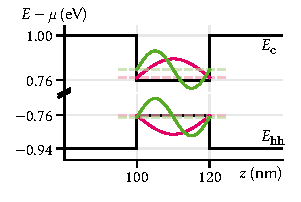
\includegraphics{img/pdf/experiment/qw_undoped_0V}
    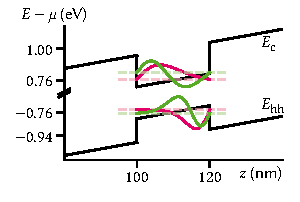
\includegraphics{img/pdf/experiment/qw_undoped_1V}
    \caption[\imgsource{img/py/experiment/qcse.py}]{
        \Gls{qcse} in an undoped \acrshort{qw}.
        Top: conduction and heavy-hole valence band profiles along the growth direction.
        The wave functions of the first two eigenstates in the well are drawn in magenta and green, respectively.
        The ground state transition is larger by $\Delta E = \qty{17}{\milli\electronvolt}$ than the gap $E_{\mr{g}}$ due to the confinement.
        Bottom: same structure as above with an out-of-plane electric field applied across the structure ($F=\qty{5}{\volt\per\micro\meter}$).
        Analytical wave functions in the infinite-well approximation are shown in magenta and green again.
        The wave functions get pushed to opposite interfaces of the \acrshort{qw}, lowering the ground state transition energy by $\Delta E = -\qty{10}{\milli\electronvolt}$.
        Excitonic effects are not included.
    }
    \label{fig:exp:theory:qcse:bandstructure}
\end{marginfigure}

Now, applying an out-of-plane electric field tilts the bands and pulls electrons and holes to opposite interfaces of the \gls{qw}.
The Hamiltonian for the electrons in this case reads~\cite{Rabinovitch1971,Miller1985,Davies2009}
\begin{equation}\label{eq:exp:theory:qcse:hamiltonian}
    H = -\frac{\hbar^2}{2m^\ast}\dv[2]{z} + eFz
\end{equation}
if we take $z$ to be zero at an interface and choose $F \geq 0$.
Introducing the length and energy scales~\cite{Davies2009}
\begin{gather}
    \tilde{\eps} = \left[\frac{\left(\hbar eF\right)^2}{2m^\ast}\right]^{\frac{1}{3}}, \\
    \tilde{z} = \left[\frac{\hbar^2}{2m^\ast eF}\right]^{\frac{1}{3}} = \frac{\tilde{\eps}}{eF},
\end{gather}
and defining
\begin{equation}
    Z_n(z) = z/\tilde{z} - \eps_n/\tilde{\eps}
\end{equation}
with $\eps_n$ the eigenvalues of $H$, the Schrödinger equation becomes~\cite{Rabinovitch1971}
\begin{equation}\label{eq:exp:theory:qcse:se}
    \dv[2]{Z_n}\psi_n(Z_n) = Z_n\psi_n(Z_n).
\end{equation}
\Cref{eq:exp:theory:qcse:se} is known as the Stokes or Airy equation and has the general solution
\begin{equation}
    \psi_n(Z_n) = \alpha_n\Ai(Z_n) + \beta_n\Bi(Z_n),
\end{equation}
where $\Ai(z)$ and $\Bi(z)$ are the Airy functions.
$\Ai(z)$ and $\Bi(z)$ oscillate for $z < 0$ and decay (grow) exponentially for $z > 0$, respectively.
As we assumed infinitely high barriers at $z = 0$ and $z = L$, the boundary conditions impose
\begin{equation}
    \psi_n(Z_n(0)) = \psi_n(Z_n(L)) = 0,
\end{equation}
which completely determines the eigenstates and -energies.
For large well widths or fields ($eFL/\eps_n\gg 1$), the second term is exponentially suppressed and the eigenenergies are given by the zeros of $\Ai(Z_n)$.
For zero field, one recovers the square well solution (\cref{eq:exp:theory:square_well:psi,eq:exp:theory:square_well:eps}).

The finite-field case is shown in the lower panel of \cref{fig:exp:theory:qcse:bandstructure} for $F=\qty{5}{\volt\per\micro\meter}$.
Due to the larger effective mass of the heavy holes, the characteristic length scale $\tilde{z}$ is shorter and hence the corresponding wave functions are narrower than their electronic counterparts.
The ground state transition energy at this field is \qty{10}{\milli\electronvolt} below the gap or \qty{27}{\milli\electronvolt} lower than in the zero-field case.

For a full quantitative accounting of the transition energies, the exciton binding energy as well as finite barrier heights would need to be included.
The former is on the order of \qtyrange{6}{9}{\milli\electronvolt} in \ch{GaAs} and becomes smaller as the overlap of the electron and hole wave functions is reduced when applying an electric field, pulling the wave functions to opposite interfaces~\cite{Miller1984}.
\Citet{Miller1985} found that finite-well properties could be reproduced by using effective well widths with infinite-well models.
The latter should have a small effect on the ground state energy as argued above.

\subsection{In-plane confinement}\label{subsec:exp:theory:qcse:trap}
% TODO: Motivate why we do all this! -> oscillator strength
So far, we have considered the \gls{qcse} in a single dimension, as if we were to apply a global electric field.
However, as we saw before, the field lowers the exciton energy below the \gls{qw} confinement and hence, if applied locally, results in an effective confinement potential in the plane of the \gls{qw}.
\citet{Descamps2021} performed numerical simulations for a geometry with circular gate electrodes with \qty{200}{\nano\meter} diameter on both sides of a membrane, finding a confinement depth of $V_0 =\qty{20}{\milli\electronvolt}$ at $F=\qty{5}{\volt\per\micro\meter}$ that is well approximated by a single-particle harmonic potential for the center-of-mass wave function of the exciton, $V(\rho) = M\omega^{2}\rho^{2}/2 - V_0$, with mass $M = m^\ast_{\mr{c}} + m^\ast_{\mr{hh}}$ and confinement strength $\omega/2\pi = \qty{738}{\giga\hertz}$ corresponding to an oscillator length $\xi=\sqrt{\hbar/M\omega}=\qty{20}{\nano\meter}$.
To obtain a qualitative picture, let us interpolate this result for different fields.
The depth of confinement corresponds to the energy shift induced by the \gls{qcse} and is quadratic in $F$, $V_0 = -\alpha F^2$.
At vanishing field, there should be no in-plane potential, $\omega=0$.
Hence, we can assume that $\omega\propto F$ to leading order and thus $V(\rho) = \beta M F^{2} \rho^{2}/2 - \alpha F^{2}$.

How does this in-plane confinement modify the wave function?
We ignore the relative motion of electron and hole as the optical properties of the exciton are dominated by the behavior at zero separation for $a_{\mr{B}}/\xi < 1$~\cite{Kavokin1994}, and consider only $\Delta n = 0$ transitions, \ie, electron and hole in the same $z$ quantum state, as $\Delta n\neq 0$ transitions are much weaker~\cite{Davies2009}.
Let us further initially assume a separable wave function and choose cylindrical coordinates according to the symmetry of the potential.
We then have
\begin{equation}\label{eq:exp:theory:qcse:trap:psi}
    \Psi_{np\ell}(z_{\mr{e}}, z_{\mr{h}}, \rho, \phi) = \psi_n(z_{\mr{e}})\psi_n(z_{\mr{h}})\chi_{p\ell}(\rho)\exp(i\ell\phi)
\end{equation}
where\sidenote{
    Note that \citeauthor{Karimi2014} miss a factor $2\pi$ in the normalization.
}~\cite{Karimi2014}
\begin{equation}\label{eq:exp:theory:qcse:trap:ho:psi}
    \chi_{p\ell}(\rho, \phi) = \sqrt{\frac{2p!}{2\pi\xi^2(p + \abs{\ell})!}}\exp(-\tilde{\rho}^2/2)\tilde{\rho}^{\abs{\ell}}L_p^{\abs{\ell}}\left(\tilde{\rho}\right)
\end{equation}
with the associated Laguerre polynomial $L_p^{\abs{\ell}}(x)$ and we used the shorthand $\tilde{\rho} = \rho/\xi$.
The numbers $p\in\mathbb{N}$ and $\ell\in\mathbb{Z}$ denote the principal and orbital momentum quantum numbers.
The eigenenergies of the harmonic oscillator solution, \cref{eq:exp:theory:qcse:trap:ho:psi}, are given by
\begin{equation}\label{eq:exp:theory:qcse:trap:ho:eps}
    \eps_{p\ell} = \hbar\omega\left(2p + \abs{\ell} + 1\right).
\end{equation}
To account for a finite well width ($L\approx\xi$ in our case), we can to a first approximation perform the replacement $\rho\to r = \sqrt{\rho^2 + z^2}$ in \cref{eq:exp:theory:qcse:trap:psi}.
The resulting wave function $\Psi_{np\ell}(r, z_{\mr{h}})$ at fixed electron coordinate $z_{\mr{e}}$ is shown in \cref{fig:exp:theory:qcse:wf} for $n = \ell = 0$ (which makes it independent of $\phi$).
For $\ell=0$ $\Psi_{np\ell}$ has $n$ nodes along $z$ and $p$ nodes along $\rho$.

\begin{figure}
    \centering
    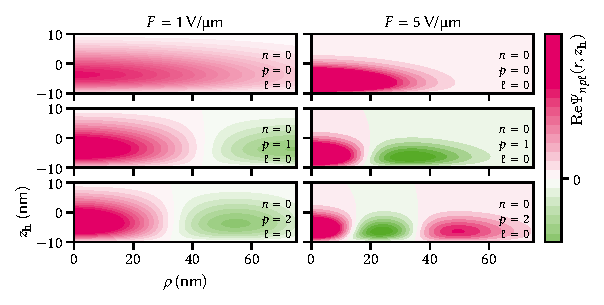
\includegraphics{img/pdf/experiment/wavefunction}
    \caption[\imgsource{img/py/experiment/qcse.py}]{
        Center-of-mass exciton wave function (hole sector) in a harmonic trap under an electric field.
        Left column shows the low-field and right column the high-field case.
        Top row is the ground state, middle and bottom row the first and second excited state in the plane, respectively.
        The out-of-plane wave function is the ground state in all cases ($n=0$) and the trap confinement strength $\omega/2\pi = \qty{738}{\giga\hertz}$ for $F=\qty{5}{\volt\per\micro\meter}$~\cite[Section~2.2.2]{Descamps2021} and linearly interpolated for \qty{1}{\volt\per\micro\meter} (see text).
    }
    \label{fig:exp:theory:qcse:wf}
\end{figure}

At last, we can use the exciton wave function $\Psi_{nm\ell}(r, \phi, z_{\mr{e}}, z_{\mr{h}})$ to estimate the \emph{oscillator strength}, a quantity often quoted in semiconductor spectroscopy.
The oscillator strength puts in relation the quantum mechanical transition rate with the emission rate of a classical oscillator with frequency $\omega = \Delta E/\hbar$ matching the transition energy~\cite{Hilborn1982}.
For a dipole transition from state $\ket{i}$ to state $\ket{j}$, it may be written as~\cite{Davies2009}
\begin{equation}
    f_{ji} = \frac{2\mu\Delta E_{ji}}{\hbar^2} \abs{\!\matrixelement{j}{\bvec{r}}{i}}^2,
\end{equation}
where $\mu$ is the reduced mass of the exciton.
As the selection rules only allow in-plane dipole transitions for heavy holes, we write~\cite{Kavokin1994}
\begin{subequations}\label{eq:exp:oscillator_strength}
    \begin{equation}\tag{\ref{eq:exp:oscillator_strength}}
        f_{np\ell} = \frac{2\mu\eps_{np\ell}}{\hbar^2} J_{r}^2 J_{\phi}^2 \abs{\!\matrixelement*{u_{\mr{c}}}{x}{u_{\mr{hh}}}}^2
    \end{equation}
    for transitions with $\Delta n = \Delta p = \Delta\ell = 0$, where
    \begin{align}
        J_{r} &= \int_{0}^{L}\dd{z}\int_0^{\infty}\dd{\rho}\rho\psi_n\gth{\mr{e}}(z)\psi_n\gth{\mr{h}}(z)\chi_{p\ell}(\sqrt{\rho^2 + z^2}), \label{eq:exp:theory:osc:rz} \\
        J_{\phi} &= \int_0^{2\pi}\dd{\phi}\exp(\i\ell\phi), \label{eq:exp:theory:osc:phi} \\
        \eps_{np\ell} &= \eps_n + \eps_{p\ell},
    \end{align}
\end{subequations}
and $\ket*{u_{\mr{c}(\mr{hh})}}$ are the Bloch functions of the valence and conduction band, respectively, that we have neglected so far.
From \cref{eq:exp:theory:osc:phi}, we immediately see that the oscillator strength of states with nonzero orbital momentum ($\ell\neq 0$) vanishes, $f_{np0}=0$!
This in turn implies from \cref{eq:exp:theory:qcse:trap:ho:eps} that the exciton level spacing in a radially symmetric trap is given by $\Delta E = 2\hbar\omega=\qty{1}{\milli\electronvolt}$, a factor of two larger than assumed by \citet{Descamps2021}.

As we tilt the bands, energy levels below the \gls{qw} become available in the barrier once $\Delta E_{\mr{c}(\mr{hh})} - \eps_{n}\sim eFd$ with $d$ the width of the barrier.
This allows confined carriers to escape the \gls{qw} with a finite probability by tunneling through the barrier, an effect known as Fowler-Nordheim tunneling.
Following \citer{Davies2009}, we can estimate the tunneling probability as\sidenote{
    The same result up to a slightly different numerical prefactor in the exponent is obtained more formally from the WKB approximation~\cite{Descamps2021}.
}
\begin{equation}\label{eq:exp:theory:qcse:tunneling:probability}
    \mathscr{T}_n(F) \approx \exp\left\lbrace -\frac{\sqrt{4 m^\ast [\Delta E_{\mr{c}(\mr{hh})} - \eps_n]^3}}{e F\hbar}\right\rbrace.
\end{equation}
The tunneling rate $\Gamma_n$ can then be estimated by the frequency that a confined charge carrier \enquote{visits} the edge of the \gls{qw} multiplied by the probability that it tunnels, $\mathscr{T}_n$~\cite{Larsson1988}.
That is, we take $\eps_n$ to be a kinetic energy and calculate the velocity as
\begin{equation}
    v_n = \frac{\hbar k_n}{m^\ast_{\mr{c}(\mr{hh})}} = \sqrt{\frac{2 \eps_n}{m^\ast_{\mr{c}(\mr{hh})}}}.
\end{equation}
Then the frequency of one round trip inside the \gls{qw} is
\begin{equation}
    \tau_n\inverse = \frac{v_n}{2L} = \frac{1}{L}\sqrt{\frac{\eps_n}{2 m^\ast_{\mr{c}(\mr{hh})}}}
\end{equation}
and
\begin{equation}\label{eq:exp:theory:qcse:tunneling:rate}
    \Gamma_n = \frac{\mathscr{T}_n}{\tau_n}.
\end{equation}
What is the order of magnitude of $\tau_n$?
For an energy of $\eps_n = \qty{10}{\milli\electronvolt}$, $\tau_n\approx\qty{200}{\femto\second}$ for electrons and \qty{400}{\femto\second} for holes.
The tunneling probability $\mathscr{T}_n$ therefore needs to be quite small indeed for the rate $\Gamma_n$ to remain small.

\begin{marginfigure}
    \centering
    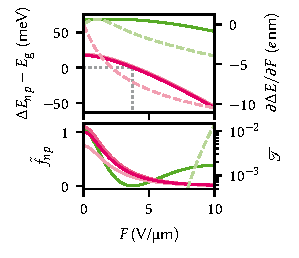
\includegraphics{img/pdf/experiment/qcse_field_dependence}
    \caption[\imgsource{img/py/experiment/qcse.py}]{
        Electric field dependence of the \gls{qcse} for the first two energy levels in the \gls{qw}.
        Top: the ground state energy (magenta) shows the expected quadratic dependence; the confinement energy is compensated at around $F=\qty{3.7}{\volt\per\micro\meter}$.
        Higher in-plane orbital levels are shown for the \gls{qw} ground state in decreasing saturation.
        For zero field, the splitting is zero as there is no in-plane confinement.
        At maximum field, the splitting is $2\hbar\omega = \qty{2}{\milli\electronvolt}$.
        Dashed lines (right axis) show the derivative, revealing that the \gls{qw} excited state is actually raised in energy at low fields.
        Bottom: oscillator strengths (same color code as above).
        Dashed lines (right axis) show the electron tunneling rate through the barrier, dash-dotted the holes.
    }
    \label{fig:exp:theory:qcse:field}
\end{marginfigure}

\Cref{fig:exp:theory:qcse:field} summarizes the \gls{qcse} in a \gls{qw} additionally confined in the plane by local electric fields.
The top panel shows the exciton transition energy $\Delta E_{np}$ for $\Delta n = \Delta p = 0$ in solid lines.\sidenote{
    Note again that we neglected the exciton binding energy, which decreases with increasing field and hence slightly reduces the redshift~\cite{Miller1984}.
}
The first three in-plane sublevels due to the harmonic potential are drawn in less saturated colors but hard to see because the level spacing is much smaller than the out-of-plane \gls{qw} subband spacing, $\sim\qty{1}{\milli\electronvolt}/\qty{50}{\milli\electronvolt}$.
The ground state shows the expected quadratic dependence on the electric field also obtained, for example, from perturbation theory.
Drawn as a dashed line is the induced dipole moment,
\begin{equation}
    \bvec{p}_{np}(F) = \pdv{\Delta E_{np}}{F}\ubvec{z},
\end{equation}
which is monotonously decreasing for the ground state as function of electric field $F$, consistent with a continuous lowering of energy.
For the first excited state, the induced dipole moment is actually positive below \qty{2}{\volt\per\micro\meter}, leading to a repulsive interaction and hence a raising of the transition energy by up to \qty{1}{\milli\electronvolt}.
The lower panel shows the oscillator strength, \cref{eq:exp:oscillator_strength}, normalized to its value of the ground state at zero field, $f_{00}(F=0)$.
For the ground state it decays exponentially with the electric field as the overlap between electron and hole wave functions, which decay exponentially into the \gls{qw} themselves, is reduced.
$f_{0p}$ for higher in-plane orbital states ($p > 0$, magenta, decreasing saturation) has an envelope following the ground state's exponential decay but vanishes at $p$ points in $F$ due to the fact that the wave function has $p$ nodes.
By contrast, $f_{10}$ for the first excited \gls{qw} state (green) does not decay to zero at large fields but also has a zero at an intermediate field because of the wave function's node along $z$.

Finally, the right axis shows the estimated tunneling rates (\cref{eq:exp:theory:qcse:tunneling:rate}) of the electron (hole) ground (excited) states in dashed (dash-dotted) magenta (green) lines, respectively.
Rates of electrons are at least four orders of magnitude larger than those of holes owing to their smaller effective mass despite the larger band offset.
At $F=\qty{5}{\volt\per\micro\meter}$ corresponding to a voltage of \qty{1}{\volt} across a membrane of \qty{200}{\nano\meter} thickness, the electron tunnel rate is on the order of \qty{1}{\hertz}, but rises very quickly above that.
Considering once again a \gls{qw} hosting a \gls{2deg} and neglecting associated band bending effects, this rate corresponds to a current through a circular area of \qty{1}{\micro\meter} in diameter of \qty{600}{\atto\ampere} at an electron density of $n = \qty{5e11}{\per\centi\meter\squared}$, but already \qty{600}{\pico\ampere} at \qty{7.5}{\volt\per\micro\meter}.

\section{Excitonic complexes}\label{sec:exp:theory:complexes}
If we liken the exciton to a Hydrogen atom\sidenote{Although positronium is a better analogon.} with modified binding energy $E_{\mr{b}}$ and Bohr radius $a_{\mr{B}}$, it is natural to expect molecules and ions of these states to exist.
The simplest molecule, or excitonic complex, is the biexciton, the analog of the \ch{H2} molecule.
Following a similar argument as for the binding energy of the exciton, we expect that of the biexciton to also increase as the dimensionality of the system is reduced.
Indeed, in \glspl{qw} it has been measured to be on the order of \qty{1}{\milli\electronvolt}, \numrange{3}{4} times larger than in 3D~\cite{Miller1985a}, although also negative binding energies, corresponding to an anti-bonding state, have been reported~\cite{Kako2004,Dialynas2008,Amloy2011}.
A signature of biexcitons is the power dependence of their \gls{pl}.
The steady-state density of electron-hole pairs, which is proportional to the exciton density at low enough powers, is proportional to the irradiance, \ie, the excitation power.
Conversely, the probability to form a two-body bound state is proportional to the square of the density of those bodies and we hence expect the power under the \gls{pl} peak of a biexciton emission to be proportional to the square of the laser power used to excite the sample.

Besides the neutral biexciton, there exist also charged states consisting of three or more bodies.
Here, additional electrons or holes bind to an exciton, forming negative or positively charged trions similar to \ch{H-} or \ch{He+} ions.
Naturally, this process is favored when a large number of surplus charge carriers is present in the sample such as is the case in doped \glspl{qw} with a \gls{2deg} (or \gls{2dhg})~\cite{Finkelstein1995}.
In these structures, the trion binding energy has been found to also be on the order of \qty{1}{\milli\electronvolt}~\cite{Esser2000,Bar-Joseph2005}.